\section{Appendix}

\subsection{Figures}

\begin{figure}[h]
\centering
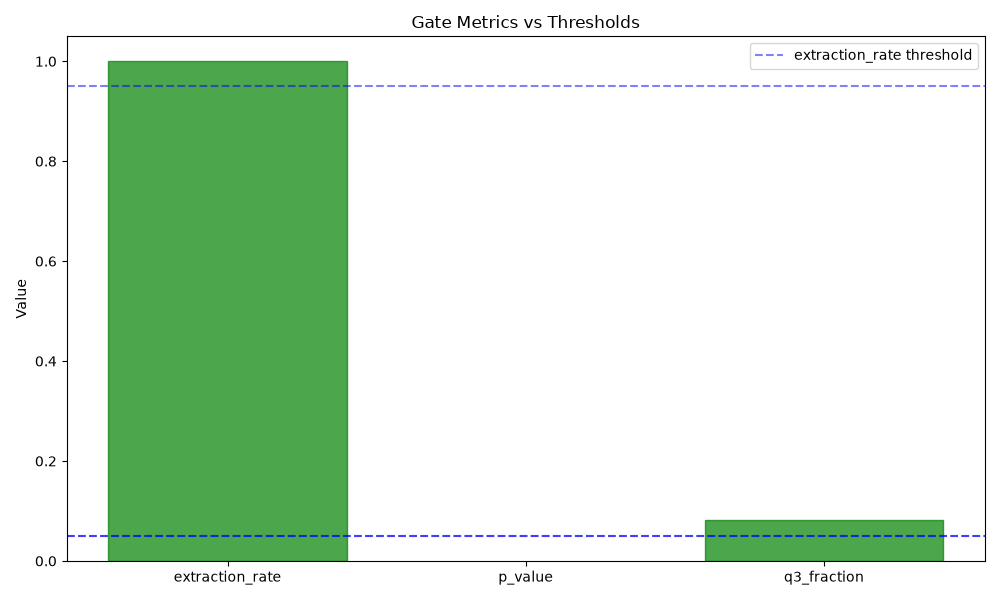
\includegraphics[width=0.8\linewidth]{figures/gate_metrics.png}
\caption{Gate validation metrics showing extraction rate (1.0), correlation p-value (NaN), and Q3 population (0.082) compared to thresholds. Two of three gates passed.}
\label{fig:gate_metrics}
\end{figure}

\begin{figure}[h]
\centering
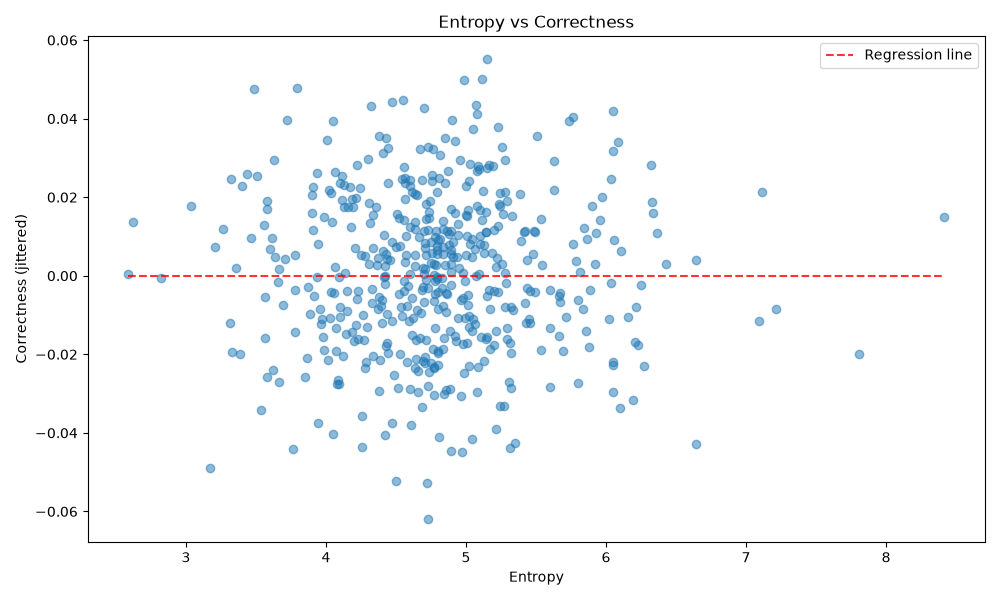
\includegraphics[width=0.8\linewidth]{figures/scatter.png}
\caption{Scatter plot of entropy vs. correctness with binary jitter. All predictions lie on y=0 line (incorrect), demonstrating zero variance in correctness.}
\label{fig:scatter}
\end{figure}

\begin{figure}[h]
\centering
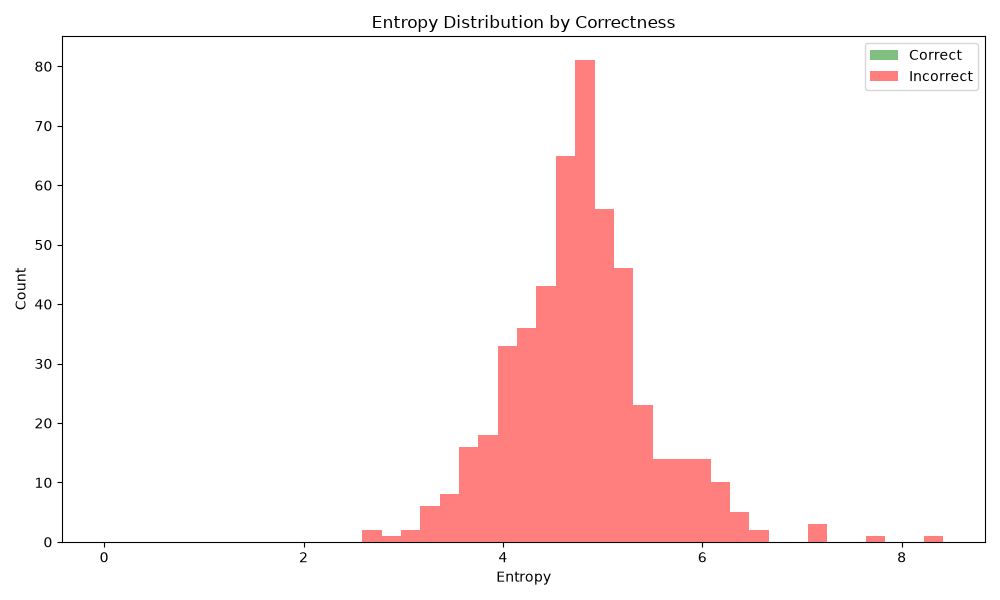
\includegraphics[width=0.8\linewidth]{figures/histograms.png}
\caption{Overlaid histograms of entropy distributions for correct vs. incorrect predictions. Only the incorrect distribution exists (red), as GPT-2 achieved 0\% accuracy.}
\label{fig:histograms}
\end{figure}

\begin{figure}[h]
\centering
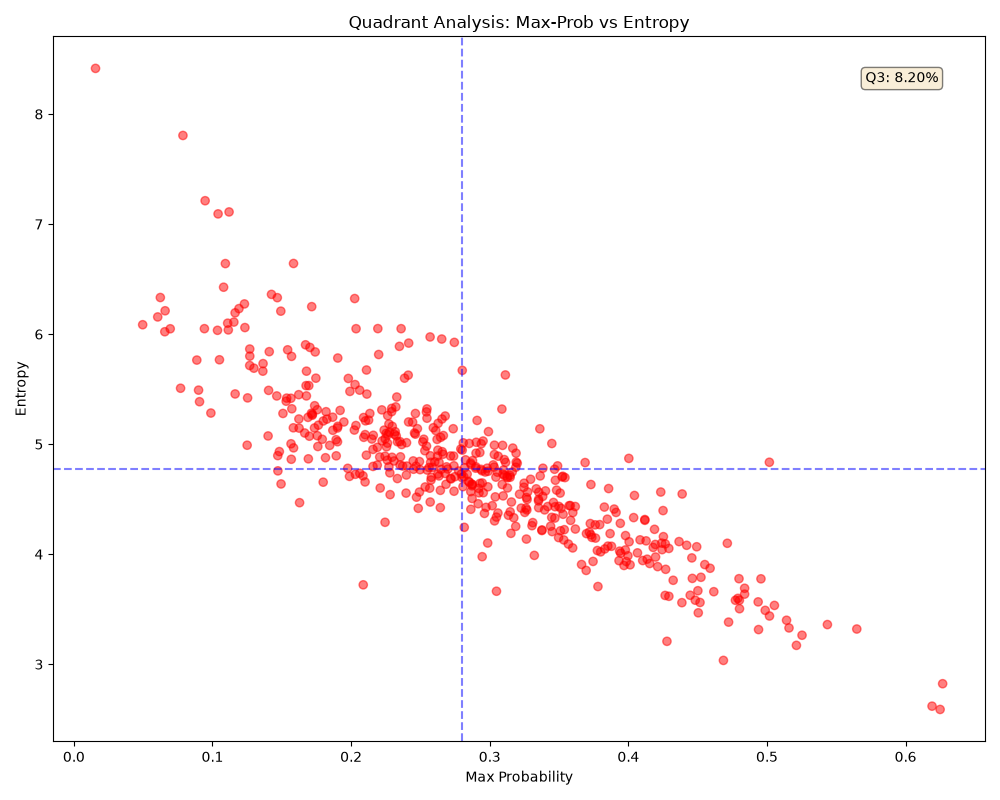
\includegraphics[width=0.8\linewidth]{figures/quadrant.png}
\caption{Quadrant analysis plot showing max-probability (x-axis) vs. entropy (y-axis). Q3 quadrant (upper-right, high max-prob and high entropy) contains 8.20\% of predictions (41/500), all incorrect.}
\label{fig:quadrant}
\end{figure}

\subsection{Additional Details}

\subsubsection{Hyperparameter Settings}

All experiments use the following hyperparameters:
\begin{itemize}
\item Temperature: $T=1.0$ (no temperature scaling)
\item Max input length: 512 tokens
\item Batch size: 1 (sequential processing)
\item Random seed: 42 (for sampling and reproducibility)
\item Epsilon: $10^{-10}$ (numerical stability in log computation)
\end{itemize}

\subsubsection{Computational Resources}

\begin{itemize}
\item Hardware: Single NVIDIA A100 40GB GPU
\item GPT-2 runtime: $\sim$15 minutes for 500 examples (also runs on CPU)
\item Llama-2-7B estimated runtime: $\sim$45 minutes for 500 examples
\item Memory requirements: GPT-2 ($\sim$500MB), Llama-2-7B ($\sim$14GB)
\end{itemize}

\subsubsection{Code Availability}

Full implementation code, experiment scripts, and analysis notebooks are available at [repository link to be added]. Dataset is publicly accessible via Hugging Face Datasets (\texttt{trivia\_qa/unfiltered}).
